\chapter{Modelagem UML do Sistema}
\label{cap:modelagem-uml}

A Linguagem de Modelagem Unificada (UML) permite representar perspectivas complementares de um sistema, como sua estrutura, seus atores e o comportamento observado durante a execução de processos. Segundo \textcite{Guedes2018}, os diagramas UML auxiliam a especificação e a comunicação dos elementos relevantes de uma solução sem pretender reproduzir cada detalhe da implementação.

Neste capítulo, os modelos foram revistos a partir do código-fonte das ramificações principais dos repositórios \textit{civitas-backend} e \textit{civitas-frontend} \parencite{CivitasBackend2026,CivitasFrontend2026}, consultados em setembro de 2026. O backend foi considerado a fonte de verdade para entidades, relacionamentos, contratos HTTP, autenticação e regras de negócio; o frontend foi utilizado para confirmar páginas, operações de interface, consultas, filtros, paginação, exportação e painel gerencial. Essa decisão evita que telas ainda não sustentadas pela API sejam apresentadas como funcionalidades concluídas.

\section{Diagrama de Classes}
\label{sec:diagrama-classes}

O Diagrama de Classes apresenta a visão estática consolidada do domínio do Civitas. A Figura~\ref{fig:diagrama-classes-civitas-atualizado}, fornecida pela equipe do projeto, registra entidades administrativas, financeiras e de auditoria, seus atributos, enumerações e multiplicidades. Controllers, Services, DTOs e Repositories não aparecem nessa figura porque representam componentes arquiteturais, e não entidades do domínio persistido.

\begin{figure}[p]
	\centering
	\caption{Diagrama de Classes do sistema Civitas}
	\label{fig:diagrama-classes-civitas-atualizado}
	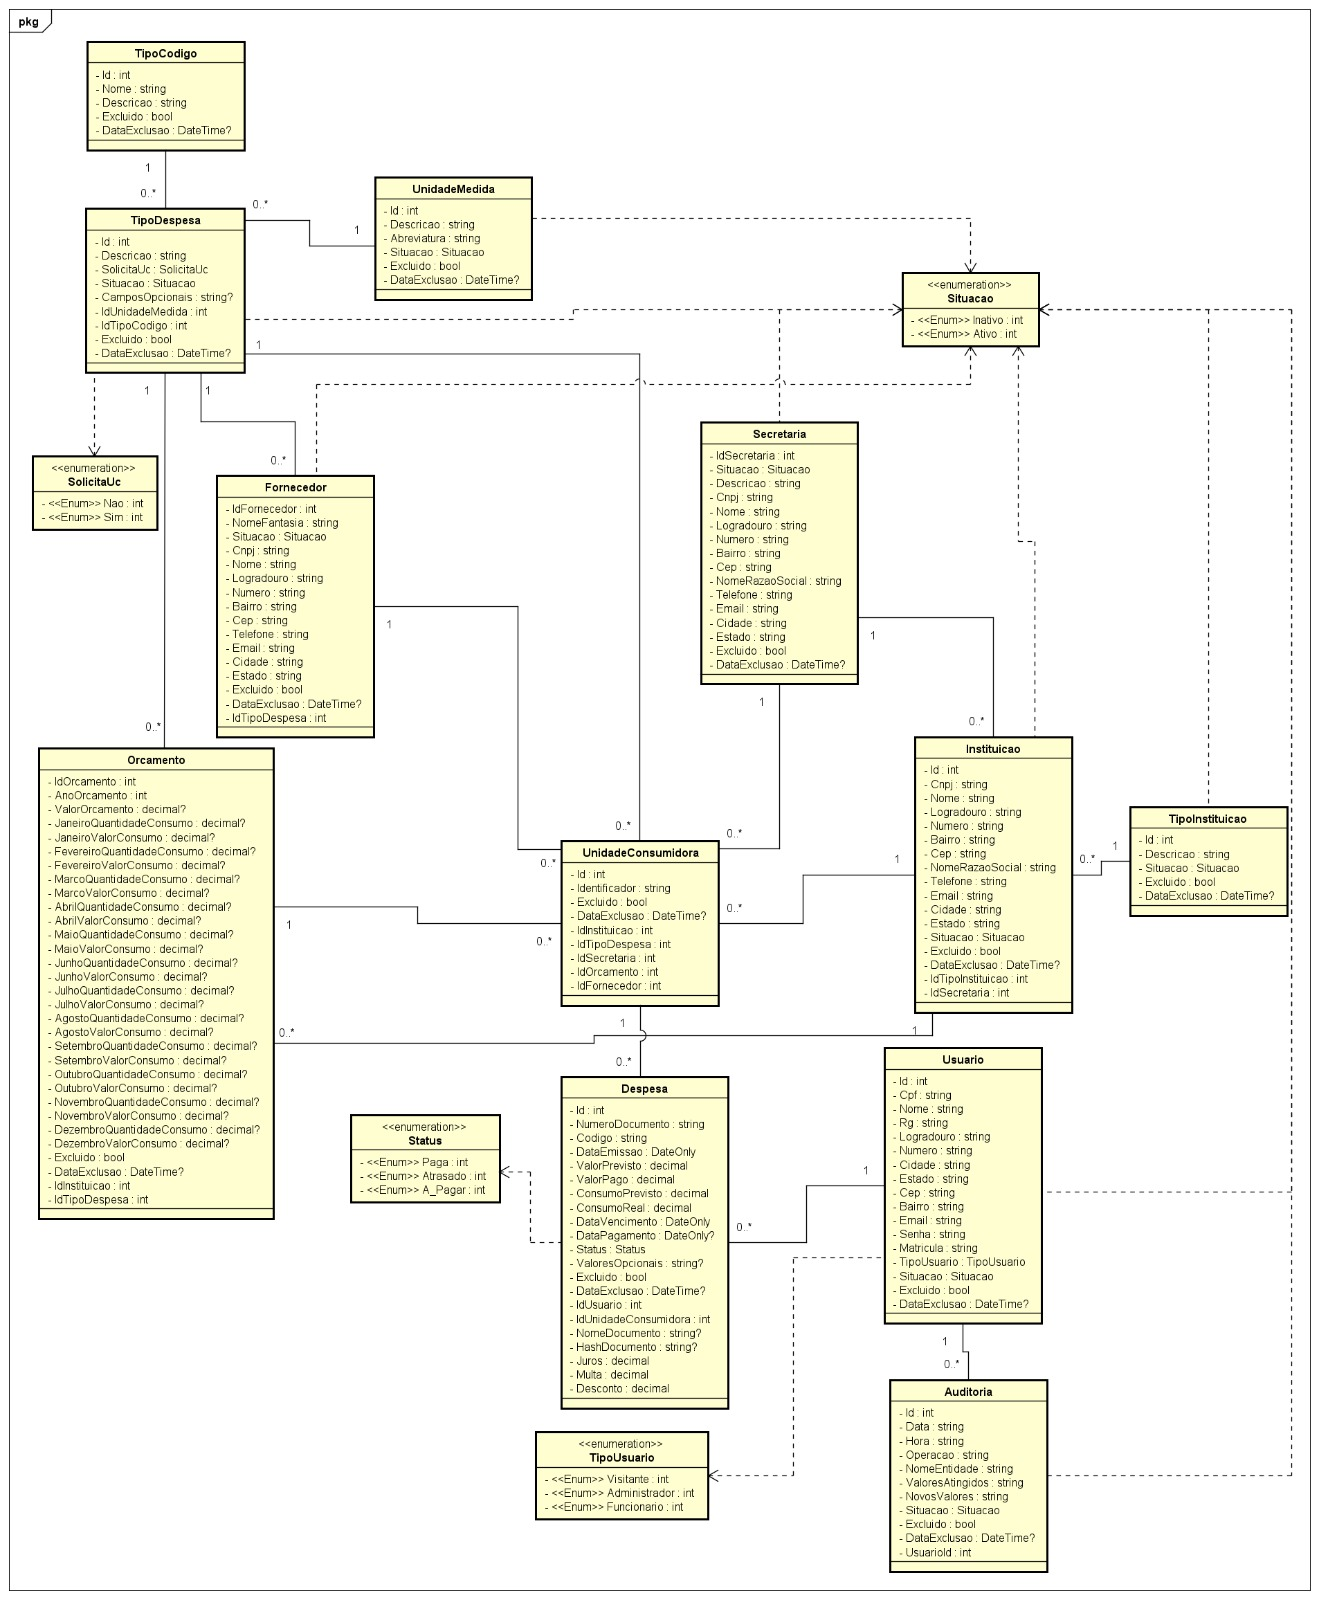
\includegraphics[width=\textwidth,height=0.82\textheight,keepaspectratio]{figs/Diagrama_Classes_Civitas.png}
	\fonte{Elaborado pelos autores com base no código-fonte do Civitas (2026).}
\end{figure}

A estrutura administrativa inicia-se em \textit{Secretaria}: cada secretaria pode manter nenhuma ou várias instituições, enquanto cada \textit{Instituicao} referencia exatamente uma secretaria e um \textit{TipoInstituicao}. A instituição, por sua vez, pode possuir orçamentos e despesas. Cada \textit{Orcamento} pertence a uma instituição e a um \textit{TipoDespesa}; cada \textit{Despesa} referencia obrigatoriamente uma instituição, um orçamento, um tipo de despesa, um fornecedor e o usuário responsável.

\textit{TipoDespesa} utiliza uma \textit{UnidadeMedida} e define, por meio de \textit{SolicitaUc}, se o preenchimento da unidade consumidora é necessário. O modelo fornecido também representa \textit{TipoCodigo} e \textit{UnidadeConsumidora}, conceitos utilizados no frontend para organizar códigos de consumo e seus vínculos com instituições, secretarias, fornecedores e orçamentos.

\textit{Fluxo} registra valor pago, consumo e estado financeiro. Um fluxo pode possuir documentos, e cada \textit{Documento} referencia um fluxo e um fornecedor. O código atual não declara associação entre \textit{Fluxo} e \textit{Despesa}; por isso, essa ligação não foi inferida no diagrama. \textit{Auditoria} referencia o \textit{Usuario} responsável e armazena a operação, a entidade afetada e os valores anteriores e posteriores. As enumerações \textit{Situacao}, \textit{SolicitaUc}, \textit{Status} e \textit{TipoUsuario} restringem os estados aceitos pelas entidades.

\section{Dicionário de Classes}
\label{sec:dicionario-classes}

O dicionário a seguir reproduz os nomes e tipos declarados nas classes C\# do backend. Chaves estrangeiras são identificadas explicitamente, e propriedades de navegação e coleções são descritas porque materializam os relacionamentos apresentados na Figura~\ref{fig:diagrama-classes-civitas-atualizado}.

\newcommand{\dicionariocivitas}[3]{%
{\small
\begin{longquadro}{|P{0.25\textwidth}|P{0.20\textwidth}|P{0.45\textwidth}|}
	\caption{Dicionário de dados de #1}
	\label{#2}\\
	\hline
	\textbf{Atributo} & \textbf{Tipo} & \textbf{Descrição} \\ \hline
	\endfirsthead
	\multicolumn{3}{c}{Quadro~\thequadro{} -- continuação} \\
	\hline
	\textbf{Atributo} & \textbf{Tipo} & \textbf{Descrição} \\ \hline
	\endhead
	\multicolumn{3}{r}{\textit{Continua na próxima página}}\\
	\endfoot
	\hline
	\multicolumn{3}{l}{\textit{Fonte: elaborado pelos autores com base no código-fonte do Civitas (2026).}}\\
	\endlastfoot
	#3
\end{longquadro}
}}

\dicionariocivitas{Secretaria}{quad:dict-secretaria}{
IdSecretaria & int & Chave primária da secretaria. \\ \hline
Situacao & Situacao & Indica se o cadastro está ativo ou inativo. \\ \hline
Descricao & string & Descrição institucional da secretaria. \\ \hline
Cnpj & string & CNPJ da secretaria. \\ \hline
Nome & string & Nome de exibição da secretaria. \\ \hline
Logradouro & string & Logradouro da sede. \\ \hline
Numero & string & Número do endereço. \\ \hline
Bairro & string & Bairro da sede. \\ \hline
Cep & string & Código de Endereçamento Postal. \\ \hline
NomeRazaoSocial & string & Razão social. \\ \hline
Email & string & E-mail institucional. \\ \hline
Telefone & string & Telefone de contato. \\ \hline
Cidade & string & Cidade da sede. \\ \hline
Estado & string & Unidade federativa. \\ \hline
Instituicoes & ICollection$<$Instituicao$>$ & Instituições subordinadas à secretaria. \\
}

\dicionariocivitas{TipoInstituicao}{quad:dict-tipo-instituicao}{
Id & int & Chave primária do tipo de instituição. \\ \hline
Descricao & string & Nome ou descrição da categoria. \\ \hline
Situacao & Situacao & Indica se a categoria está ativa ou inativa. \\ \hline
Instituicoes & ICollection$<$Instituicao$>$ & Instituições classificadas por este tipo. \\
}

\dicionariocivitas{Instituicao}{quad:dict-instituicao}{
Id & int & Chave primária da instituição. \\ \hline
CNPJ & string & CNPJ da instituição. \\ \hline
Nome & string & Nome de exibição. \\ \hline
Logradouro & string & Logradouro do endereço. \\ \hline
Numero & string & Número do endereço. \\ \hline
Bairro & string & Bairro. \\ \hline
CEP & string & Código de Endereçamento Postal. \\ \hline
NomeRazaoSocial & string & Razão social. \\ \hline
Telefone & string & Telefone de contato. \\ \hline
Email & string & E-mail institucional. \\ \hline
Cidade & string & Cidade. \\ \hline
Estado & string & Unidade federativa. \\ \hline
Situacao & Situacao & Indica se o cadastro está ativo ou inativo. \\ \hline
IdTipoInstituicao & int & Chave estrangeira obrigatória de TipoInstituicao. \\ \hline
TipoInstituicao & TipoInstituicao & Navegação para a categoria da instituição. \\ \hline
IdSecretaria & int & Chave estrangeira obrigatória de Secretaria. \\ \hline
Secretaria & Secretaria & Navegação para a secretaria responsável. \\ \hline
Orcamento & ICollection$<$Orcamento$>$ & Orçamentos associados à instituição. \\ \hline
Despesas & ICollection$<$Despesa$>$ & Despesas associadas à instituição. \\
}

\dicionariocivitas{UnidadeMedida}{quad:dict-unidade-medida}{
Id & int & Chave primária da unidade de medida. \\ \hline
Descricao & string & Nome completo da unidade. \\ \hline
Abreviatura & string & Símbolo ou abreviatura. \\ \hline
Situacao & Situacao & Indica se a unidade está ativa ou inativa. \\ \hline
TiposDespesas & ICollection$<$TipoDespesa$>$ & Tipos de despesa que utilizam a unidade. \\
}

\dicionariocivitas{TipoDespesa}{quad:dict-tipo-despesa}{
Id & int & Chave primária do tipo de despesa. \\ \hline
Descricao & string & Descrição da categoria de gasto. \\ \hline
IdUnidadeMedida & int & Chave estrangeira obrigatória de UnidadeMedida. \\ \hline
UnidadeMedida & UnidadeMedida & Navegação para a unidade utilizada. \\ \hline
SolicitaUc & SolicitaUc & Define se a UC deve ser informada na despesa. \\ \hline
Situacao & Situacao & Indica se o tipo está ativo ou inativo. \\ \hline
Despesas & ICollection$<$Despesa$>$ & Despesas classificadas por este tipo. \\
}

\dicionariocivitas{Fornecedor}{quad:dict-fornecedor}{
IdFornecedor & int & Chave primária do fornecedor. \\ \hline
NomeFantasia & string & Nome fantasia. \\ \hline
Situacao & Situacao & Indica se o cadastro está ativo ou inativo. \\ \hline
Cnpj & string & CNPJ único do fornecedor. \\ \hline
Nome & string & Razão social ou nome cadastral. \\ \hline
Logradouro & string & Logradouro do endereço. \\ \hline
Numero & string & Número do endereço. \\ \hline
Bairro & string & Bairro. \\ \hline
Cep & string & Código de Endereçamento Postal. \\ \hline
Telefone & string & Telefone de contato. \\ \hline
Email & string & E-mail de contato. \\ \hline
Cidade & string & Cidade. \\ \hline
Estado & string & Unidade federativa. \\ \hline
Documentos & ICollection$<$Documento$>$ & Documentos emitidos pelo fornecedor. \\ \hline
Despesas & ICollection$<$Despesa$>$ & Despesas vinculadas ao fornecedor. \\
}

\dicionariocivitas{Orcamento}{quad:dict-orcamento}{
IdOrcamento & int & Chave primária do orçamento. \\ \hline
AnoOrcamento & int & Exercício do orçamento. \\ \hline
ValorOrcamento & double & Valor planejado. \\ \hline
IdInstituicao & int & Chave estrangeira obrigatória de Instituicao. \\ \hline
Instituicao & Instituicao? & Navegação para a instituição responsável. \\ \hline
IdTipoDespesa & int & Chave estrangeira obrigatória de TipoDespesa. \\ \hline
TipoDespesa & TipoDespesa? & Navegação para a categoria orçamentária. \\ \hline
Despesas & ICollection$<$Despesa$>$ & Despesas que consomem o orçamento. \\
}

\dicionariocivitas{Despesa}{quad:dict-despesa}{
Id & int & Chave primária da despesa. \\ \hline
NumeroDocumento & string & Número obrigatório do documento; deve conter somente dígitos. \\ \hline
UC & string & Código textual da unidade consumidora, obrigatório conforme TipoDespesa. \\ \hline
DataEmissao & string & Data de emissão normalizada pelo serviço para dia-mês-ano. \\ \hline
ConsumoPrevisto & double & Quantidade de consumo prevista, não negativa. \\ \hline
DataVencimento & DateOnly & Data de vencimento, igual ou posterior à emissão. \\ \hline
Situacao & Situacao & Indica se o registro está ativo ou inativo. \\ \hline
IdTipoDespesa & int & Chave estrangeira obrigatória de TipoDespesa. \\ \hline
TipoDespesa & TipoDespesa & Navegação para a categoria da despesa. \\ \hline
IdOrcamento & int & Chave estrangeira obrigatória de Orcamento. \\ \hline
Orcamento & Orcamento & Navegação para o orçamento utilizado. \\ \hline
IdInstituicao & int & Chave estrangeira obrigatória de Instituicao. \\ \hline
Instituicao & Instituicao & Navegação para a instituição responsável. \\ \hline
IdFornecedor & int & Chave estrangeira obrigatória de Fornecedor. \\ \hline
Fornecedor & Fornecedor & Navegação para o fornecedor. \\ \hline
IdUsuario & int & Chave estrangeira obrigatória de Usuario. \\ \hline
Usuario & Usuario & Navegação para o autor do lançamento. \\
}

\dicionariocivitas{Fluxo}{quad:dict-fluxo}{
IdFluxo & int & Chave primária do fluxo financeiro. \\ \hline
ValorPago & float & Valor efetivamente pago. \\ \hline
Consumo & int & Consumo realizado. \\ \hline
Status & Status & Estado financeiro do fluxo. \\ \hline
Documentos & ICollection$<$Documento$>$ & Documentos vinculados ao fluxo. \\
}

\dicionariocivitas{Documento}{quad:dict-documento}{
IdDocumento & int & Chave primária do documento. \\ \hline
Digitalizacao & byte[] & Conteúdo binário digitalizado. \\ \hline
NumeroDocumento & int & Número de identificação do documento. \\ \hline
IdFornecedor & int & Chave estrangeira obrigatória de Fornecedor. \\ \hline
Fornecedor & Fornecedor & Navegação para o emissor. \\ \hline
IdFluxo & int & Chave estrangeira obrigatória de Fluxo. \\ \hline
Fluxo & Fluxo & Navegação para o fluxo comprovado. \\
}

\dicionariocivitas{Usuario}{quad:dict-usuario}{
Id & int & Chave primária do usuário. \\ \hline
Cpf & string & CPF único do usuário. \\ \hline
Nome & string & Nome completo. \\ \hline
Rg & string & Registro Geral. \\ \hline
Logradouro & string & Logradouro residencial. \\ \hline
Numero & string & Número do endereço. \\ \hline
Cidade & string & Cidade. \\ \hline
Estado & string & Unidade federativa. \\ \hline
Cep & string & Código de Endereçamento Postal. \\ \hline
Bairro & string & Bairro. \\ \hline
Email & string & E-mail único utilizado no login. \\ \hline
Senha & string & Hash da senha gerado com BCrypt. \\ \hline
Matricula & string & Matrícula única do usuário. \\ \hline
TipoUsuario & TipoUsuario & Perfil nominal do cadastro. \\ \hline
Situacao & Situacao & Determina se o acesso está liberado. \\ \hline
Despesas & ICollection$<$Despesa$>$ & Despesas lançadas pelo usuário. \\
}

\dicionariocivitas{Auditoria}{quad:dict-auditoria}{
Id & int & Chave primária do registro de auditoria. \\ \hline
Data & string & Data informada para a ocorrência. \\ \hline
Hora & string & Horário informado para a ocorrência. \\ \hline
Operacao & string & Operação executada. \\ \hline
NomeEntidade & string & Entidade afetada. \\ \hline
ValoresAtingidos & string & Valores anteriores ou atingidos. \\ \hline
NovosValores & string & Valores resultantes da operação. \\ \hline
Situacao & Situacao & Indica se o registro está ativo ou inativo. \\ \hline
UsuarioId & int & Chave estrangeira obrigatória de Usuario. \\ \hline
Usuario & Usuario? & Navegação para o responsável pela ocorrência. \\
}

\dicionariocivitas{enumeração Situacao}{quad:dict-enum-situacao}{
ATIVO & int (1) & Cadastro disponível para uso. \\ \hline
INATIVO & int (2) & Cadastro indisponível para novas operações. \\
}

\dicionariocivitas{enumeração SolicitaUc}{quad:dict-enum-solicita-uc}{
Sim & int (1) & Exige o preenchimento de UC na despesa. \\ \hline
Não & int (2) & Não exige o preenchimento de UC. \\
}

\dicionariocivitas{enumeração Status}{quad:dict-enum-status}{
a\_pagar & int (1) & Fluxo ainda pendente de pagamento. \\ \hline
paga & int (2) & Fluxo pago. \\ \hline
atrasado & int (3) & Fluxo em atraso. \\
}

\dicionariocivitas{enumeração TipoUsuario}{quad:dict-enum-tipo-usuario}{
VISITANTE & int (1) & Perfil nominal visitante. \\ \hline
ADMINISTRADOR & int (2) & Perfil nominal administrador. \\ \hline
FUNCIONARIO & int (3) & Perfil nominal funcionário. \\
}

\iffalse
\section{Definição de Atores}
\label{sec:definicao-atores}

Os atores representam papéis externos que interagem com o sistema, e não componentes internos da aplicação. O código define os valores Visitante, Administrador e Funcionário na enumeração \textit{TipoUsuario}. Entretanto, na versão examinada, todas as rotas de negócio utilizam apenas o atributo \texttt{[Authorize]}, sem políticas ou restrições por papel, e o frontend também não oculta páginas conforme o tipo do usuário. Assim, os três perfis especializam o ator \textit{Usuário autenticado} e possuem tecnicamente o mesmo alcance depois do login. Essa constatação é importante para que o modelo descreva o software atual, sem atribuir controles ainda não implementados.

\begin{quadro}[H]
	\centering
	\caption{Definição dos atores do Civitas}
	\label{quad:atores-civitas}
	\small
	\begin{tabularx}{\textwidth}{|p{0.20\textwidth}|X|X|}
		\hline
		\textbf{Ator} & \textbf{Responsabilidade no domínio} & \textbf{Permissões e limitações implementadas} \\ \hline
		Administrador & Perfil destinado à administração dos cadastros, usuários, configurações e rotinas financeiras. & Precisa possuir cadastro ativo e autenticar-se. O tipo é transportado no JWT, mas ainda não restringe endpoints ou páginas. \\ \hline
		Funcionário & Perfil operacional destinado à manutenção cotidiana de instituições, fornecedores, orçamentos, despesas, fluxos e documentos. & Submete-se às mesmas exigências de autenticação do administrador; não há autorização técnica que limite seu acesso a um subconjunto. \\ \hline
		Visitante & Perfil nominal de acesso limitado previsto pela enumeração do domínio. & Quando possui conta ativa e se autentica, recebe o mesmo acesso técnico aos recursos protegidos. Não existe área pública de consulta nem regra RBAC específica no código atual. \\ \hline
	\end{tabularx}
	\fonte{Elaborado pelos autores com base no código-fonte do Civitas (2026).}
\end{quadro}

\begin{figure}[H]
	\centering
	\caption{Diagrama de Atores do sistema Civitas}
	\label{fig:atores-civitas-atualizado}
	\includegraphics[width=0.92\textwidth]{figs/Atores_Civitas_Atualizado.png}
	\fonte{Elaborado pelos autores com base no código-fonte do Civitas (2026).}
\end{figure}

\section{Casos de Uso}
\label{sec:casos-uso}

Os casos de uso foram derivados dos controllers da API e das páginas e operações efetivamente disponíveis no frontend. O termo \textit{gerenciar} reúne as operações implementadas para cada recurso, que podem variar entre cadastrar, listar, consultar, atualizar e alterar situação. A exclusão física não é atribuída quando o controller oferece apenas alternância entre \textit{ATIVO} e \textit{INATIVO}.

\small
\begin{longquadro}{|p{0.07\textwidth}|p{0.20\textwidth}|p{0.25\textwidth}|p{0.38\textwidth}|}
	\caption{Casos de uso comuns aos usuários autenticados}
	\label{quad:casos-uso-autenticados}\\
	\hline
	\textbf{ID} & \textbf{Caso de uso} & \textbf{Entrada principal} & \textbf{Resposta esperada} \\ \hline
	\endfirsthead
	\multicolumn{4}{c}{Quadro~\thequadro{} -- continuação} \\
	\hline
	\textbf{ID} & \textbf{Caso de uso} & \textbf{Entrada principal} & \textbf{Resposta esperada} \\ \hline
	\endhead
	UC01 & Realizar login & E-mail e senha & Token JWT, expiração e identificação do usuário ativo. \\ \hline
	UC02 & Encerrar sessão & Ação de saída & Dados locais da sessão removidos e retorno ao login. \\ \hline
	UC03 & Consultar painel gerencial & Sessão autenticada & Indicadores, despesas recentes e vencimentos apresentados pela interface. \\ \hline
	UC04 & Consultar perfil & Identificador do usuário da sessão & Dados cadastrais e tipo de usuário. \\ \hline
	UC05 & Gerenciar usuários & Dados pessoais, endereço, matrícula, perfil e situação & Cadastro, consulta, atualização ou alteração de situação. \\ \hline
	UC06 & Gerenciar secretarias & Dados institucionais, endereço e situação & Cadastro, listagem paginada, consulta, atualização ou alteração de situação. \\ \hline
	UC07 & Gerenciar instituições & Dados institucionais, secretaria e tipo de instituição & Cadastro, consulta por ID ou nome, atualização ou alteração de situação. \\ \hline
	UC08 & Gerenciar fornecedores & Dados fiscais, endereço, contato e situação & Cadastro validado, consulta, atualização ou alteração de situação. \\ \hline
	UC09 & Gerenciar configurações & Tipo de instituição, tipo de despesa ou unidade de medida & Manutenção dos cadastros auxiliares e de suas situações. \\ \hline
	UC10 & Gerenciar orçamentos & Ano, valor, instituição e tipo de despesa & Cadastro, consulta e atualização do orçamento. \\ \hline
	UC11 & Gerenciar despesas & Documento, datas, consumo, UC e referências & Cadastro validado, consulta, atualização ou alteração de situação. \\ \hline
	UC12 & Gerenciar fluxos financeiros & Valor pago, consumo e status & Cadastro, consulta, atualização ou alteração do status. \\ \hline
	UC13 & Gerenciar documentos & Digitalização, número, fornecedor e fluxo & Cadastro, consulta ou atualização do documento. \\ \hline
	UC14 & Consultar auditorias & Paginação ou filtros de usuário, entidade e operação & Registros de auditoria correspondentes. \\ \hline
	UC15 & Consultar listagens & Busca, filtros, ordenação, colunas e página & Recorte solicitado apresentado na tabela ou em cartões. \\ \hline
	UC16 & Exportar listagem & Formato PDF ou XLSX e visualização atual & Arquivo gerado no navegador com dados e colunas selecionados. \\
	\hline
	\multicolumn{4}{l}{\textit{Fonte: elaborado pelos autores com base no código-fonte do Civitas (2026).}}\\
\end{longquadro}
\normalsize

O Quadro~\ref{quad:casos-uso-por-ator} relaciona os casos aos três perfis. A igualdade técnica entre as linhas não é uma regra de negócio proposta: ela documenta a ausência atual de RBAC. Uma evolução futura deverá adicionar políticas no backend e proteção equivalente no frontend antes que permissões distintas possam ser afirmadas.

\begin{quadro}[H]
	\centering
	\caption{Casos de uso disponíveis por ator na implementação atual}
	\label{quad:casos-uso-por-ator}
	\small
	\begin{tabularx}{\textwidth}{|p{0.20\textwidth}|X|}
		\hline
		\textbf{Ator} & \textbf{Casos de uso disponíveis} \\ \hline
		Administrador & UC01 a UC16, desde que o cadastro esteja ativo e a requisição autenticada. \\ \hline
		Funcionário & UC01 a UC16, nas mesmas condições técnicas do administrador. \\ \hline
		Visitante & UC01 a UC16 quando possui conta ativa; o código não implementa restrição adicional para este valor de perfil. \\ \hline
	\end{tabularx}
	\fonte{Elaborado pelos autores com base no código-fonte do Civitas (2026).}
\end{quadro}

\section{Diagrama de Casos de Uso}
\label{sec:diagrama-casos-uso}

O diagrama geral da Figura~\ref{fig:casos-uso-geral-civitas} utiliza generalização para evitar repetir associações idênticas dos três perfis. As relações \textit{include} aparecem somente quando o comportamento é obrigatório, como validar o JWT antes de acessar recursos protegidos e validar dados ao manter despesas. A exportação é modelada como extensão da consulta de listagens, pois ocorre opcionalmente a partir de uma visualização já preparada.

\begin{figure}[p]
	\centering
	\caption{Diagrama Geral de Casos de Uso do sistema Civitas}
	\label{fig:casos-uso-geral-civitas}
	\includegraphics[width=\textwidth,height=0.82\textheight,keepaspectratio]{figs/Casos_Uso_Geral_Civitas.png}
	\fonte{Elaborado pelos autores com base no código-fonte do Civitas (2026).}
\end{figure}

O login é a única operação pública da API. Depois de autenticado, o ator pode acessar os módulos administrativos e financeiros, as listagens e o perfil. O encerramento de sessão é executado no cliente pela remoção dos dados persistidos no navegador. O painel, os filtros e a exportação são comportamentos da aplicação web; já os cadastros e consultas são suportados pelos endpoints REST correspondentes.

\section{Diagrama de Casos de Uso -- Individuais}
\label{sec:casos-uso-individuais}

Foram selecionados autenticação e cadastro de despesa porque concentram regras que justificam detalhamento individual. Operações puramente repetitivas de listagem e atualização permanecem no diagrama geral.

\subsection{Caso de Uso Individual -- Autenticar Usuário}

\begin{quadro}[H]
	\centering
	\caption{Especificação do caso de uso UC01 -- Realizar login}
	\label{quad:uc-login}
	\small
	\begin{tabularx}{\textwidth}{|p{0.22\textwidth}|X|}
		\hline
		\textbf{Elemento} & \textbf{Especificação} \\ \hline
		Ator & Usuário (Administrador, Funcionário ou Visitante). \\ \hline
		Objetivo & Obter uma sessão autenticada para acessar o ambiente interno. \\ \hline
		Pré-condições & O usuário deve estar cadastrado, ativo e possuir senha armazenada em formato de hash BCrypt. \\ \hline
		Fluxo principal & 1. O usuário informa e-mail e senha; 2. a interface envia os dados; 3. o serviço valida e normaliza os campos; 4. o repositório localiza o usuário; 5. o serviço confirma situação ativa e senha; 6. o sistema emite o JWT; 7. a interface armazena a sessão e abre o painel. \\ \hline
		Fluxos alternativos & A1: campo ausente gera erro de validação. A2: usuário inexistente, inativo ou senha incorreta gera resposta 401 sem informar qual condição falhou. \\ \hline
		Pós-condições & Token válido emitido com identificador, nome e tipo do usuário, acompanhado do horário de expiração. \\ \hline
	\end{tabularx}
	\fonte{Elaborado pelos autores com base no código-fonte do Civitas (2026).}
\end{quadro}

\begin{figure}[H]
	\centering
	\caption{Diagrama individual do caso de uso Autenticar Usuário}
	\label{fig:uc-individual-login}
	\includegraphics[width=0.96\textwidth]{figs/UC_Autenticar_Usuario.png}
	\fonte{Elaborado pelos autores com base no código-fonte do Civitas (2026).}
\end{figure}

\subsection{Caso de Uso Individual -- Cadastrar Despesa}

\begin{quadro}[H]
	\centering
	\caption{Especificação do caso de uso UC11 -- Cadastrar despesa}
	\label{quad:uc-cadastrar-despesa}
	\small
	\begin{tabularx}{\textwidth}{|p{0.22\textwidth}|X|}
		\hline
		\textbf{Elemento} & \textbf{Especificação} \\ \hline
		Ator & Usuário autenticado. \\ \hline
		Objetivo & Registrar uma obrigação financeira com suas referências administrativas e orçamentárias. \\ \hline
		Pré-condições & Token válido; tipo de despesa, orçamento, instituição, fornecedor e usuário previamente cadastrados; fornecedor ativo. \\ \hline
		Fluxo principal & 1. O ator preenche documento, datas, consumo, situação e referências; 2. o serviço normaliza os textos e valida os campos; 3. consulta as entidades relacionadas; 4. verifica a coerência entre orçamento, instituição e tipo de despesa; 5. verifica duplicidade; 6. persiste a despesa; 7. retorna confirmação. \\ \hline
		Fluxos alternativos & A1: UC ausente quando o tipo exige UC. A2: data de emissão futura ou vencimento anterior à emissão. A3: referência inexistente ou fornecedor inativo. A4: orçamento incompatível com instituição ou tipo. A5: mesmo número de documento já cadastrado para o fornecedor. Em qualquer caso, a API retorna erro 400 e não grava o registro. \\ \hline
		Pós-condições & Despesa persistida e relacionada às cinco entidades informadas; nenhuma alteração ocorre quando uma validação falha. \\ \hline
	\end{tabularx}
	\fonte{Elaborado pelos autores com base no código-fonte do Civitas (2026).}
\end{quadro}

\begin{figure}[H]
	\centering
	\caption{Diagrama individual do caso de uso Cadastrar Despesa}
	\label{fig:uc-individual-despesa}
	\includegraphics[width=\textwidth]{figs/UC_Cadastrar_Despesa.png}
	\fonte{Elaborado pelos autores com base no código-fonte do Civitas (2026).}
\end{figure}

\section{Diagrama de Sequência}
\label{sec:diagramas-sequencia}

Os diagramas de sequência evidenciam a ordem das mensagens entre ator, interface, controller, service, repository e banco de dados. As alternativas de sucesso e falha foram preservadas para refletir as respostas observáveis da API.

\subsection{Autenticar Usuário}

\begin{figure}[H]
	\centering
	\caption{Diagrama de Sequência -- Autenticar Usuário}
	\label{fig:seq-login-civitas}
	\includegraphics[width=\textwidth]{figs/Sequencia_Autenticar_Usuario.png}
	\fonte{Elaborado pelos autores com base no código-fonte do Civitas (2026).}
\end{figure}

O \textit{AuthController} encaminha as credenciais ao \textit{AuthService}, que consulta o usuário por e-mail, verifica a situação e compara a senha com o hash BCrypt. Somente no fluxo válido o \textit{JwtTokenService} emite o token e a interface abre o painel.

\subsection{Cadastrar Despesa}

\begin{figure}[p]
	\centering
	\caption{Diagrama de Sequência -- Cadastrar Despesa}
	\label{fig:seq-despesa-civitas}
	\includegraphics[width=\textwidth,height=0.78\textheight,keepaspectratio]{figs/Sequencia_Cadastrar_Despesa.png}
	\fonte{Elaborado pelos autores com base no código-fonte do Civitas (2026).}
\end{figure}

O \textit{DespesaService} concentra as regras do cadastro. Antes da inserção, ele consulta os repositórios relacionados, verifica a compatibilidade do orçamento e a unicidade do número do documento por fornecedor. Uma violação encerra o fluxo com erro 400; caso contrário, o repositório persiste a entidade.

\subsection{Alterar Status de Fluxo}

\begin{figure}[H]
	\centering
	\caption{Diagrama de Sequência -- Alterar Status de Fluxo}
	\label{fig:seq-fluxo-civitas}
	\includegraphics[width=\textwidth]{figs/Sequencia_Alterar_Status_Fluxo.png}
	\fonte{Elaborado pelos autores com base no código-fonte do Civitas (2026).}
\end{figure}

O controller recebe o identificador e o novo valor de \textit{Status}. Depois de confirmar a existência do fluxo, encaminha a atualização pelas camadas de serviço e repositório. A ausência do registro produz resposta 404; a atualização confirmada retorna o novo estado.

\section{Diagrama de Atividade}
\label{sec:diagramas-atividade}

Os diagramas de atividade representam decisões e retornos que não ficam evidentes em uma lista de operações. Foram escolhidos os mesmos processos críticos detalhados nas seções anteriores, mantendo rastreabilidade entre requisitos, casos de uso e comportamento.

\begin{figure}[p]
	\centering
	\caption{Diagrama de Atividade -- Cadastrar Despesa}
	\label{fig:atividade-cadastrar-despesa}
	\includegraphics[width=\textwidth,height=0.80\textheight,keepaspectratio]{figs/Atividade_Cadastrar_Despesa.png}
	\fonte{Elaborado pelos autores com base no código-fonte do Civitas (2026).}
\end{figure}

A atividade de cadastro percorre validações de campos, datas, referências, obrigatoriedade de UC, compatibilidade orçamentária, situação do fornecedor e duplicidade documental. Cada decisão inválida conduz a uma resposta sem persistência; somente a passagem por todas as verificações permite gravar a despesa.

\begin{figure}[H]
	\centering
	\caption{Diagrama de Atividade -- Autenticação}
	\label{fig:atividade-login-civitas}
	\includegraphics[width=0.78\textwidth]{figs/Atividade_Autenticacao.png}
	\fonte{Elaborado pelos autores com base no código-fonte do Civitas (2026).}
\end{figure}

Na autenticação, campos ausentes encerram o processo com erro de validação. Credenciais inválidas ou usuário inativo resultam em resposta não autorizada; credenciais válidas produzem o JWT e o redirecionamento ao painel. O fluxo não diferencia as causas da falha de credenciais, evitando revelar se determinado e-mail está cadastrado.

\fi

\section{Definição de Atores}
\label{sec:definicao-atores-civitas-final}

Os atores do Civitas são Administrador, Funcionário e Visitante. Os três especializam o ator genérico Usuário, conforme a Figura~\ref{fig:atores-civitas-final}, mas possuem responsabilidades diferentes nos diagramas funcionais fornecidos pela equipe.

\begin{figure}[H]
	\centering
	\caption{Definição dos atores do sistema Civitas}
	\label{fig:atores-civitas-final}
	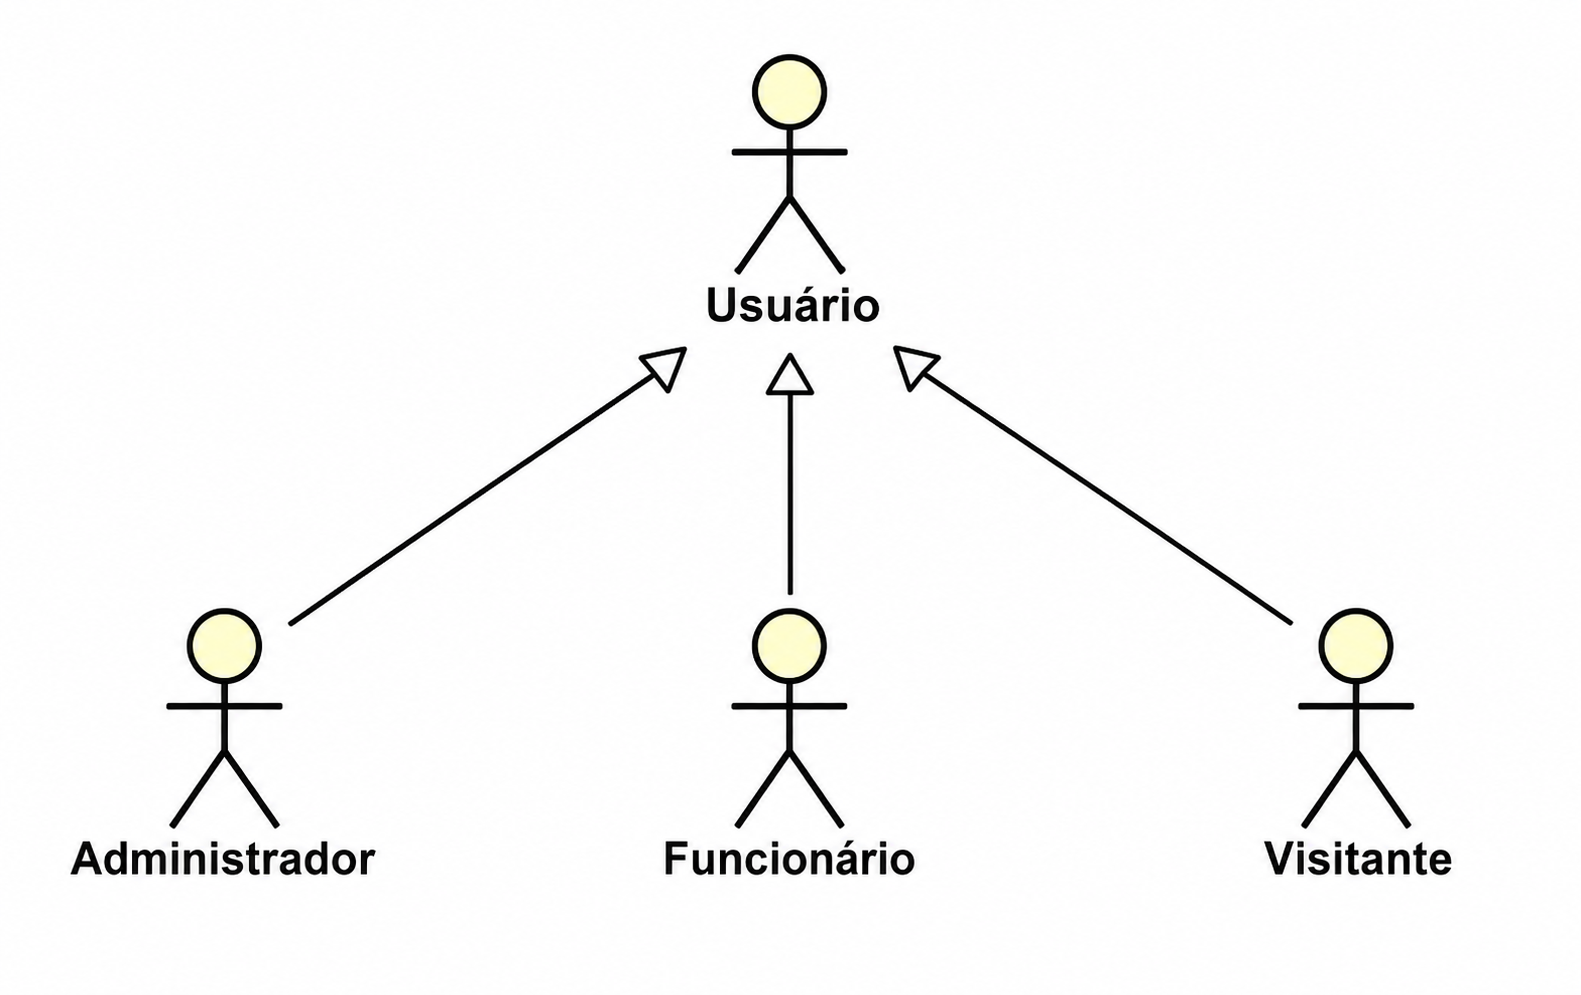
\includegraphics[width=0.92\textwidth]{figs/atores_civitas.png}
	\fonte{Elaborado pelos autores (2026).}
\end{figure}

\begin{quadro}[H]
	\centering
	\caption{Responsabilidades dos atores do Civitas}
	\label{quad:atores-civitas-final}
	\small
	\begin{tabularx}{\textwidth}{|p{0.20\textwidth}|X|X|}
		\hline
		\textbf{Ator} & \textbf{Responsabilidade} & \textbf{Limitações representadas} \\ \hline
		Administrador & Mantém usuários, secretarias, fornecedores, instituições, orçamentos, despesas e configurações; consulta e registra auditorias. & Suas operações internas dependem de autenticação e validação dos dados. \\ \hline
		Funcionário & Executa rotinas operacionais de instituições, fornecedores, despesas e unidades consumidoras, além de consultar cadastros auxiliares. & Não recebe, no diagrama fornecido, todas as operações administrativas de usuários e secretarias. \\ \hline
		Visitante & Consulta dados disponibilizados de secretarias, instituições, fornecedores, orçamentos, despesas e configurações. & Possui acesso somente às operações de listagem, consulta e carregamento representadas em seu diagrama. \\ \hline
	\end{tabularx}
	\fonte{Elaborado pelos autores com base nos diagramas do Civitas (2026).}
\end{quadro}

\section{Casos de Uso}
\label{sec:casos-uso-civitas-final}

Os casos de uso foram organizados por ator, preservando as funcionalidades dos diagramas fornecidos. Operações internas como carregar e validar representam comportamentos reutilizados durante consultas, cadastros e atualizações; elas não substituem o objetivo principal percebido pelo usuário.

\small
\begin{longquadro}{|p{0.08\textwidth}|p{0.18\textwidth}|p{0.28\textwidth}|p{0.36\textwidth}|}
	\caption{Casos de uso do Visitante}
	\label{quad:casos-uso-visitante}\\
	\hline
	\textbf{ID} & \textbf{Módulo} & \textbf{Caso de uso} & \textbf{Resultado} \\ \hline
	\endfirsthead
	\multicolumn{4}{c}{Quadro~\thequadro{} -- continuação}\\ \hline
	\textbf{ID} & \textbf{Módulo} & \textbf{Caso de uso} & \textbf{Resultado} \\ \hline
	\endhead
	VIS01 & Secretaria & Listar e consultar secretaria & Exibe os dados da secretaria selecionada. \\ \hline
	VIS02 & Instituição & Listar e consultar instituição & Exibe os dados da instituição selecionada. \\ \hline
	VIS03 & Fornecedor & Listar e consultar fornecedor & Exibe os dados do fornecedor selecionado. \\ \hline
	VIS04 & Orçamento & Listar e consultar orçamento & Exibe os dados do orçamento selecionado. \\ \hline
	VIS05 & Despesa & Listar e consultar despesa & Exibe os dados da despesa selecionada. \\ \hline
	VIS06 & Configuração & Listar e consultar tipo de despesa & Exibe o tipo de despesa selecionado. \\ \hline
	VIS07 & Configuração & Listar e consultar tipo de instituição & Exibe o tipo de instituição selecionado. \\ \hline
	VIS08 & Configuração & Listar e consultar unidade de medida & Exibe a unidade de medida selecionada. \\
	\hline
	\multicolumn{4}{l}{\textit{Fonte: elaborado pelos autores com base no diagrama do Visitante (2026).}}\\
\end{longquadro}

\begin{longquadro}{|p{0.08\textwidth}|p{0.18\textwidth}|p{0.28\textwidth}|p{0.36\textwidth}|}
	\caption{Casos de uso do Funcionário}
	\label{quad:casos-uso-funcionario-civitas}\\
	\hline
	\textbf{ID} & \textbf{Módulo} & \textbf{Caso de uso} & \textbf{Resultado} \\ \hline
	\endfirsthead
	\multicolumn{4}{c}{Quadro~\thequadro{} -- continuação}\\ \hline
	\textbf{ID} & \textbf{Módulo} & \textbf{Caso de uso} & \textbf{Resultado} \\ \hline
	\endhead
	FUN01 & Autenticação & Realizar login e logout & Inicia ou encerra a sessão do funcionário. \\ \hline
	FUN02 & Secretaria & Listar e consultar secretaria & Apresenta a secretaria solicitada. \\ \hline
	FUN03 & Fornecedor & Cadastrar, atualizar, listar e consultar fornecedor & Mantém os dados cadastrais do fornecedor. \\ \hline
	FUN04 & Instituição & Cadastrar, atualizar, listar e consultar instituição & Mantém instituições e seus vínculos. \\ \hline
	FUN05 & Orçamento & Listar e consultar orçamento & Apresenta o orçamento solicitado. \\ \hline
	FUN06 & Despesa & Cadastrar, atualizar, listar, consultar e alterar status & Mantém a despesa e permite visualizar seu documento. \\ \hline
	FUN07 & Configuração & Listar e consultar tipos de despesa e instituição & Apresenta os cadastros auxiliares solicitados. \\ \hline
	FUN08 & Configuração & Listar e consultar unidade de medida & Apresenta a unidade de medida solicitada. \\ \hline
	FUN09 & Tipo de código & Listar e consultar tipo de código & Apresenta a classificação solicitada. \\ \hline
	FUN10 & Unidade consumidora & Cadastrar, atualizar, listar e consultar unidade consumidora & Mantém o cadastro e seus relacionamentos. \\ \hline
	FUN11 & Endereço & Consultar endereço por CEP & Valida o CEP e retorna o endereço localizado. \\ \hline
	FUN12 & Auditoria & Registrar auditoria & Registra a operação executada pelo usuário. \\
	\hline
	\multicolumn{4}{l}{\textit{Fonte: elaborado pelos autores com base no diagrama do Funcionário (2026).}}\\
\end{longquadro}

\begin{longquadro}{|p{0.08\textwidth}|p{0.18\textwidth}|p{0.28\textwidth}|p{0.36\textwidth}|}
	\caption{Casos de uso do Administrador}
	\label{quad:casos-uso-administrador-civitas}\\
	\hline
	\textbf{ID} & \textbf{Módulo} & \textbf{Caso de uso} & \textbf{Resultado} \\ \hline
	\endfirsthead
	\multicolumn{4}{c}{Quadro~\thequadro{} -- continuação}\\ \hline
	\textbf{ID} & \textbf{Módulo} & \textbf{Caso de uso} & \textbf{Resultado} \\ \hline
	\endhead
	ADM01 & Autenticação & Realizar login & Autentica o administrador e gera o token de acesso. \\ \hline
	ADM02 & Usuário & Cadastrar, atualizar, listar, consultar e ativar/inativar usuário & Mantém usuários após validação. \\ \hline
	ADM03 & Secretaria & Cadastrar, atualizar, listar, consultar e ativar/inativar secretaria & Mantém secretarias após validação. \\ \hline
	ADM04 & Fornecedor & Cadastrar, atualizar, listar, consultar e ativar/inativar fornecedor & Mantém fornecedores após validação. \\ \hline
	ADM05 & Instituição & Cadastrar, atualizar, listar, consultar e ativar/inativar instituição & Mantém instituições e vínculos. \\ \hline
	ADM06 & Orçamento & Cadastrar, atualizar, listar, consultar e excluir/restaurar orçamento & Mantém o planejamento orçamentário. \\ \hline
	ADM07 & Despesa & Cadastrar, atualizar, listar, consultar, alterar status e excluir/restaurar & Mantém despesas e documentos associados. \\ \hline
	ADM08 & Configuração & Gerenciar tipos de despesa e instituição & Mantém e valida os cadastros auxiliares. \\ \hline
	ADM09 & Configuração & Gerenciar unidades de medida e tipos de código & Mantém classificações e respectivas situações. \\ \hline
	ADM10 & Unidade consumidora & Cadastrar, atualizar, listar, consultar e excluir/restaurar & Mantém unidades consumidoras após validação. \\ \hline
	ADM11 & Endereço & Consultar endereço por CEP & Valida o CEP e retorna o endereço. \\ \hline
	ADM12 & Auditoria & Consultar e registrar auditorias & Mantém a rastreabilidade das operações. \\
	\hline
	\multicolumn{4}{l}{\textit{Fonte: elaborado pelos autores com base no diagrama do Administrador (2026).}}\\
\end{longquadro}
\normalsize

\section{Diagrama de Casos de Uso}
\label{sec:diagramas-casos-uso-civitas-final}

Os diagramas fornecidos distribuem as funcionalidades conforme o alcance de cada ator. Para preservar a legibilidade, cada perfil é apresentado separadamente.

\begin{figure}[p]
	\centering
	\caption{Diagrama Geral de Casos de Uso -- Visitante}
	\label{fig:uc-geral-visitante-civitas}
	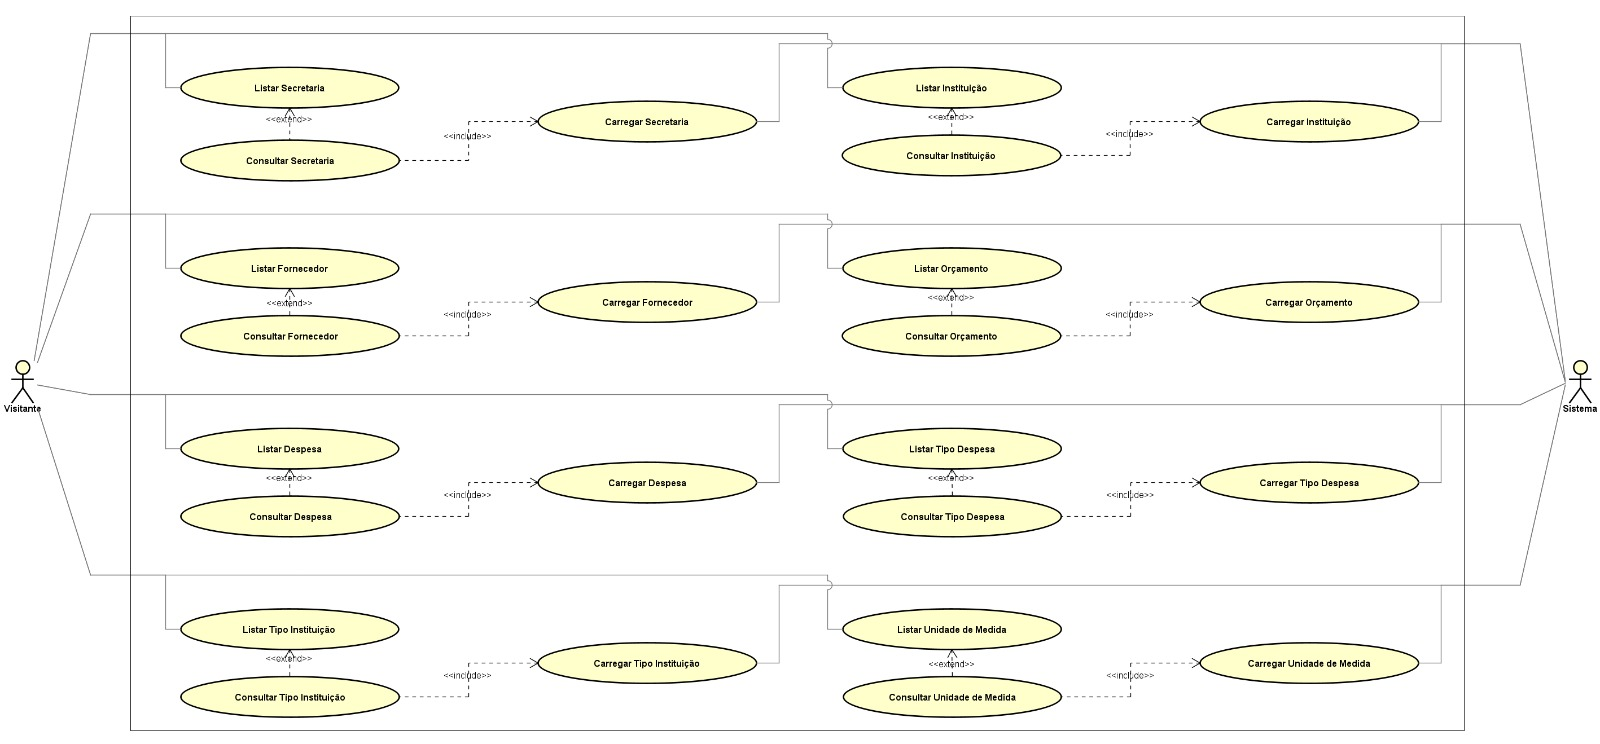
\includegraphics[width=\textwidth,height=0.80\textheight,keepaspectratio]{figs/UCGeral_Visitante_Civitas.png}
	\fonte{Elaborado pelos autores (2026).}
\end{figure}

A Figura~\ref{fig:uc-geral-visitante-civitas} concentra operações de leitura. O Visitante lista um conjunto de registros, seleciona o elemento desejado e consulta os dados carregados pelo sistema.

\begin{figure}[p]
	\centering
	\caption{Diagrama Geral de Casos de Uso -- Funcionário}
	\label{fig:uc-geral-funcionario-civitas}
	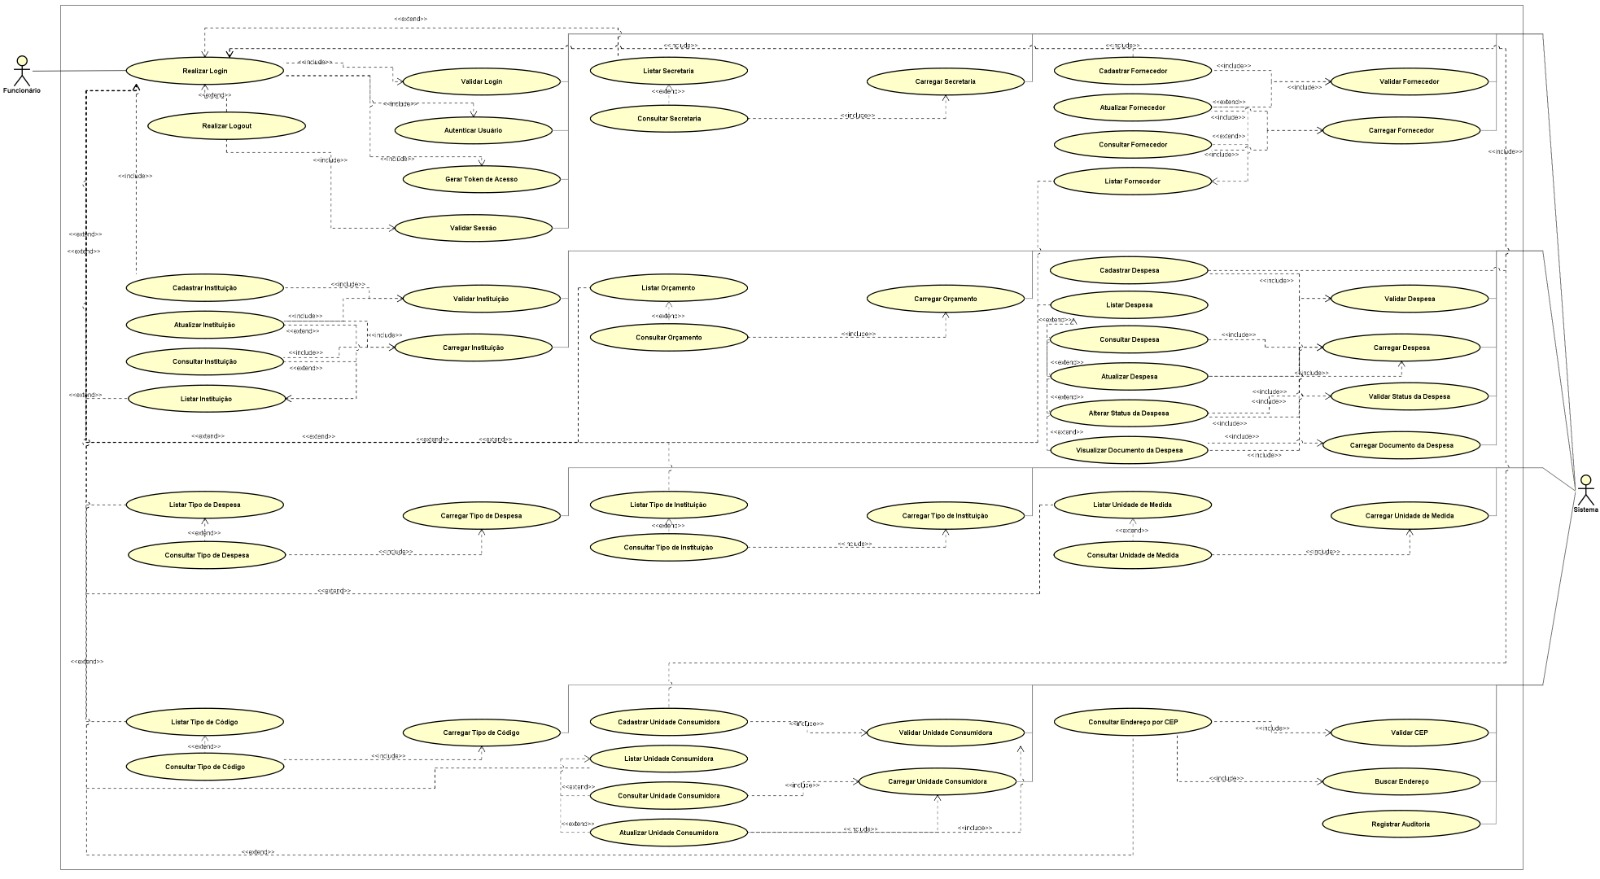
\includegraphics[width=\textwidth,height=0.80\textheight,keepaspectratio]{figs/UCGeral_Funcionario_Civitas.png}
	\fonte{Elaborado pelos autores (2026).}
\end{figure}

A Figura~\ref{fig:uc-geral-funcionario-civitas} apresenta o perfil operacional. Além da autenticação, o Funcionário mantém fornecedores, instituições, despesas e unidades consumidoras, consulta cadastros de apoio e registra auditoria.

\begin{figure}[p]
	\centering
	\caption{Diagrama Geral de Casos de Uso -- Administrador}
	\label{fig:uc-geral-administrador-civitas}
	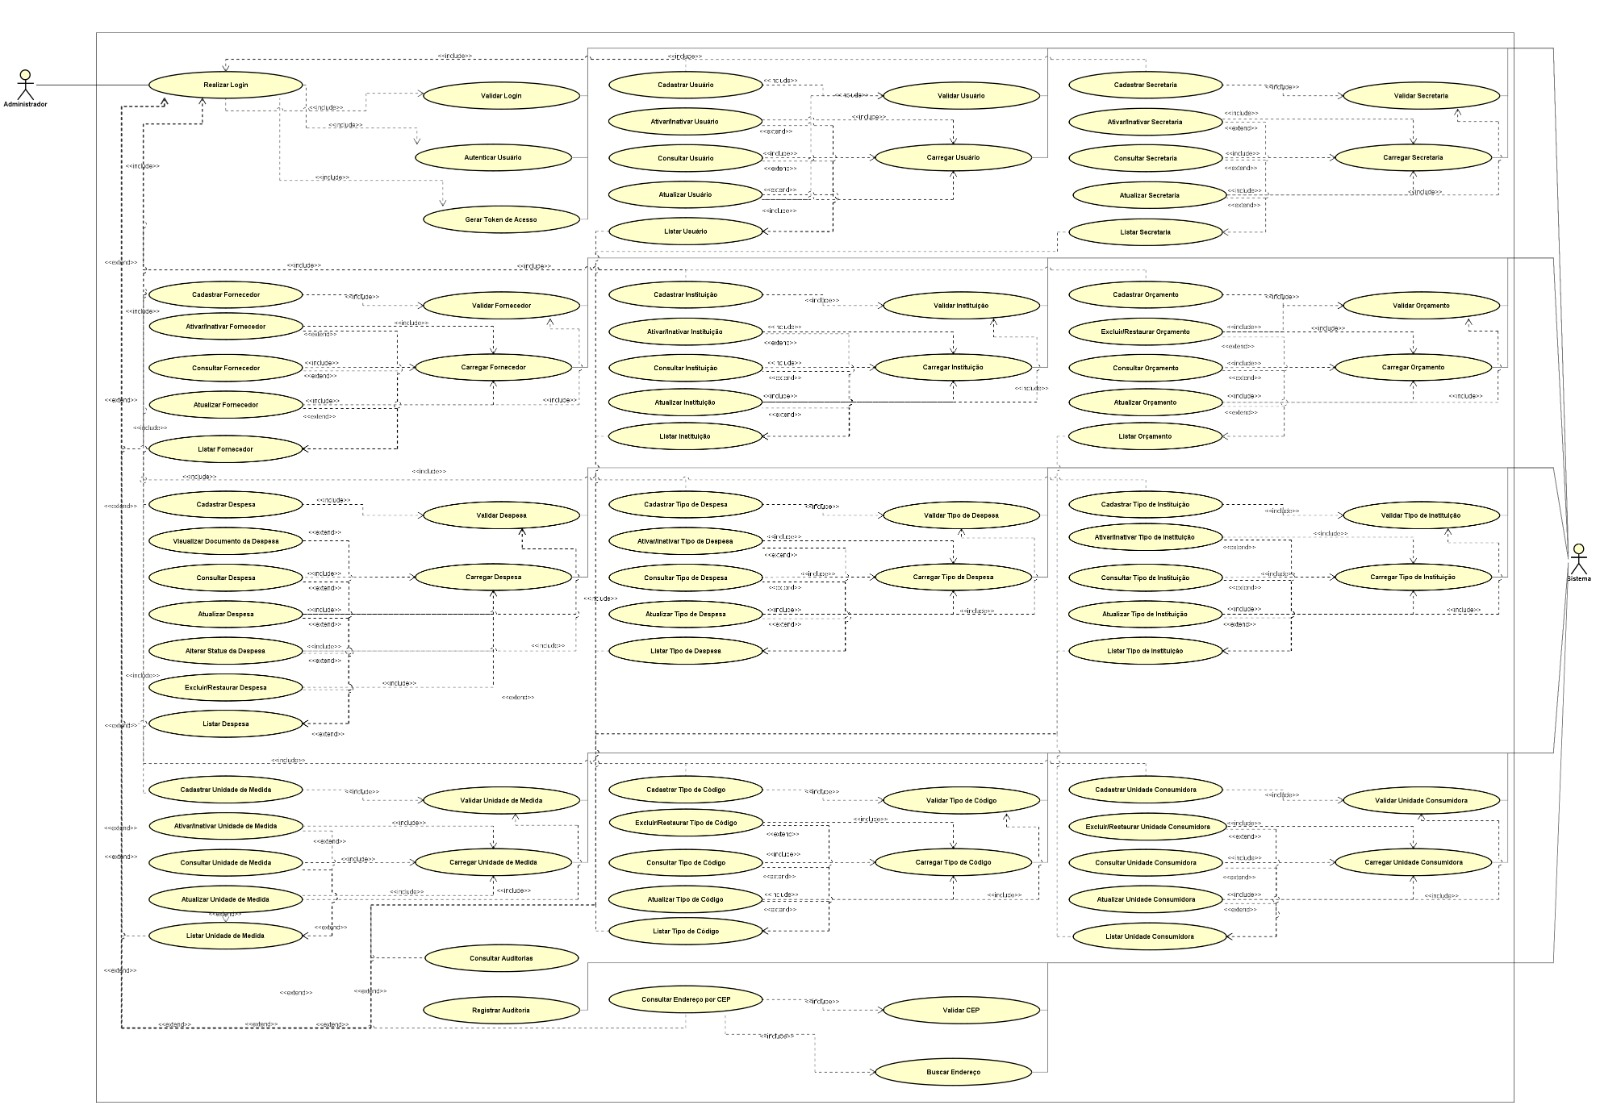
\includegraphics[width=\textwidth,height=0.80\textheight,keepaspectratio]{figs/UCGeral_Administrador_Civitas.png}
	\fonte{Elaborado pelos autores (2026).}
\end{figure}

A Figura~\ref{fig:uc-geral-administrador-civitas} reúne o maior conjunto de operações. O Administrador gerencia os cadastros centrais, controla ativações, inativações, exclusões e restaurações, consulta endereços e acompanha auditorias.

\section{Diagrama de Casos de Uso -- Individuais}
\label{sec:casos-uso-individuais-civitas-final}

O cadastro de usuário foi selecionado para detalhamento por envolver autenticação prévia, validação, verificação de duplicidade, persistência e auditoria.

\begin{quadro}[H]
	\centering
	\caption{Especificação do caso de uso individual Cadastrar Usuário}
	\label{quad:uc-cadastrar-usuario}
	\small
	\begin{tabularx}{\textwidth}{|p{0.22\textwidth}|X|}
		\hline
		\textbf{Elemento} & \textbf{Especificação} \\ \hline
		Ator & Administrador. \\ \hline
		Objetivo & Registrar um novo usuário e seu perfil de acesso no Civitas. \\ \hline
		Pré-condições & O administrador deve ter realizado login e possuir os dados obrigatórios do novo usuário. \\ \hline
		Fluxo principal & 1. O administrador inicia o cadastro; 2. informa os dados pessoais, endereço, e-mail, matrícula, senha, situação e tipo de usuário; 3. o sistema valida os campos; 4. verifica duplicidades; 5. salva o usuário; 6. registra a auditoria; 7. informa o sucesso. \\ \hline
		Fluxos alternativos & A1: dados inválidos impedem o salvamento. A2: CPF, e-mail ou matrícula já utilizados produzem mensagem de conflito. A3: falha de persistência cancela a operação e informa o erro. \\ \hline
		Pós-condições & Usuário persistido e ocorrência de auditoria registrada quando o fluxo é concluído. \\ \hline
	\end{tabularx}
	\fonte{Elaborado pelos autores com base no código-fonte e no diagrama fornecido (2026).}
\end{quadro}

\begin{figure}[H]
	\centering
	\caption{Diagrama individual do caso de uso Cadastrar Usuário}
	\label{fig:uc-individual-cadastrar-usuario}
	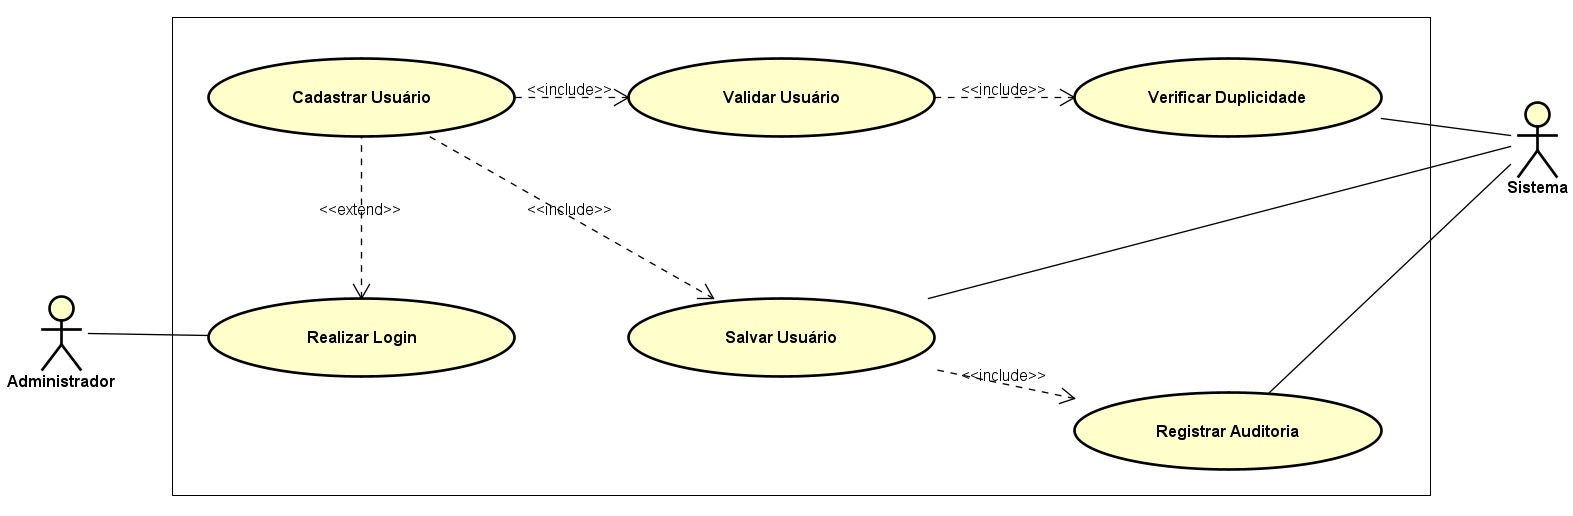
\includegraphics[width=\textwidth]{figs/UCIndividual_Cadastrar_Usuario_Civitas.png}
	\fonte{Elaborado pelos autores (2026).}
\end{figure}

\section{Diagrama de Sequência}
\label{sec:diagrama-sequencia-civitas-final}

O fluxo de cadastro de usuário inicia-se na interface utilizada pelo Administrador. A requisição é recebida pelo \textit{UsuarioController}, encaminhada ao \textit{UsuarioService} para normalização, validação dos campos e verificação de CPF, e-mail e matrícula, e então persistida pelo \textit{UsuarioRepository}. Depois da confirmação do banco de dados, a operação pode originar o registro de auditoria e a interface apresenta o resultado ao ator.

\begin{quadro}[H]
	\centering
	\caption{Sequência de interações do cadastro de usuário}
	\label{quad:sequencia-cadastrar-usuario}
	\small
	\begin{tabularx}{\textwidth}{|p{0.08\textwidth}|p{0.30\textwidth}|X|}
		\hline
		\textbf{Ordem} & \textbf{Participantes} & \textbf{Mensagem} \\ \hline
		1 & Administrador $\rightarrow$ Interface & Informa os dados e confirma o cadastro. \\ \hline
		2 & Interface $\rightarrow$ UsuarioController & Envia a requisição de criação do usuário. \\ \hline
		3 & UsuarioController $\rightarrow$ UsuarioService & Solicita a validação do cadastro. \\ \hline
		4 & UsuarioService $\rightarrow$ UsuarioRepository & Consulta possíveis duplicidades. \\ \hline
		5 & UsuarioRepository $\rightarrow$ Banco de dados & Executa as consultas por CPF, e-mail e matrícula. \\ \hline
		6 & UsuarioService $\rightarrow$ UsuarioRepository & Solicita a persistência quando os dados são válidos. \\ \hline
		7 & UsuarioRepository $\rightarrow$ Banco de dados & Insere o novo usuário. \\ \hline
		8 & UsuarioController $\rightarrow$ Interface & Retorna sucesso ou a mensagem de validação. \\ \hline
	\end{tabularx}
	\fonte{Elaborado pelos autores com base na arquitetura do Civitas (2026).}
\end{quadro}

\section{Diagrama de Atividade}
\label{sec:diagrama-atividade-civitas-final}

A Figura~\ref{fig:atividade-login-civitas-final} representa o processo de autenticação utilizado como pré-condição das operações internas. O usuário informa e-mail e senha, a API valida os dados e o fluxo segue para o módulo solicitado quando as credenciais estão corretas. Informações incorretas produzem um alerta e permitem nova tentativa.

\begin{figure}[H]
	\centering
	\caption{Diagrama de Atividade -- Realizar Login}
	\label{fig:atividade-login-civitas-final}
	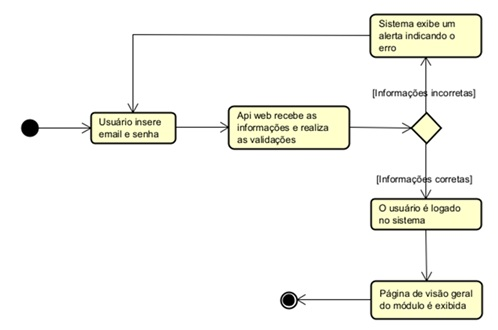
\includegraphics[width=0.78\textwidth]{figs/atividade_login.jpg}
	\fonte{Elaborado pelos autores (2026).}
\end{figure}

\let\dicionariocivitas\relax
